\documentclass[aspectratio=169]{beamer}

% ---------- ENCODING & FONTS ----------
\usepackage[utf8]{inputenc}
\usepackage[T1]{fontenc}

% ---------- THEME & LOOK ----------
\usetheme{Madrid}
\usecolortheme{seahorse}
\usefonttheme{professionalfonts}
\setbeamertemplate{navigation symbols}{}
\setbeamercovered{transparent}
\setbeamertemplate{itemize items}[circle]
\setbeamertemplate{enumerate items}[default]
\setlength{\parskip}{0.25em}

% ---------- COLORS ----------
\definecolor{accent}{RGB}{0,92,184}
\definecolor{soft}{RGB}{233,244,255}
\definecolor{canadared}{RGB}{196,30,58}
\definecolor{leafgreen}{RGB}{0,130,80}
\definecolor{goldenrod}{RGB}{218,165,32}
\definecolor{deeporange}{RGB}{220,90,20}
\definecolor{shiftpurple}{RGB}{130,50,180}
\definecolor{tealblue}{RGB}{0,128,128}
\definecolor{lightred}{RGB}{245,210,210}
\setbeamercolor{structure}{fg=accent}
\setbeamercolor{title}{fg=white,bg=accent}
\setbeamercolor{frametitle}{fg=accent}
\setbeamercolor{block title}{bg=accent!12,fg=accent}
\setbeamercolor{block body}{bg=soft}

% ---------- PACKAGES ----------
\usepackage{booktabs}
\usepackage{amsmath, amssymb}
\usepackage{array}
\usepackage{multirow}
\usepackage{hyperref}
\usepackage{tikz}
\usepackage{pgfplots}
\pgfplotsset{compat=1.18}
\usetikzlibrary{arrows.meta, positioning, calc, shapes.geometric}
\hypersetup{colorlinks=true,linkcolor=accent,urlcolor=accent}

% ---------- SAFE TRANSITION FALLBACK ----------
\makeatletter
\@ifundefined{transfade}{\newcommand{\transfade}[1][]{}}{}
\makeatother

% ---------- TITLE ----------
\title{\textbf{Money, Banks, and the Bank of Canada}}
\subtitle{{\large ECON 101 -- Principles of Macroeconomics}}
\author{Muhebullah Karimzada}
\date{Spring 2026}

% ============================================================
\begin{document}
% ============================================================

\begin{frame}[plain]
  \titlepage
\end{frame}

\begin{frame}{Chapter Outline}
\transfade
\begin{itemize}
  \item \textbf{10.1} What Is Money, and Why Do We Need It?
  \item \textbf{10.2} How Is Money Measured in Canada Today?
  \item \textbf{10.3} How Do Banks Create Money?
  \item \textbf{10.5} The Quantity Theory of Money
\end{itemize}
\end{frame}

% ============================================================
\section{10.1 What Is Money, and Why Do We Need It?}
% ============================================================

\begin{frame}{10.1 Learning Objective}
\transfade
\begin{block}{Goal}
Define money and discuss the four functions of money.
\end{block}
\begin{itemize}
  \item \textbf{Money:} any asset people generally accept in exchange for goods/services or to settle debts.
  \item Money is one of humanity's most important inventions:
  \begin{itemize}
    \item enables specialization and trade,
    \item supports development of complex economies.
  \end{itemize}
  \item \textbf{Canada today:} physical cash accounts for $<$10\% of transactions; the rest are digital (debit, Interac, credit, e-transfer).
\end{itemize}
\end{frame}

\begin{frame}{Life Without Money: The Problem with Barter}
\transfade
\begin{itemize}
  \item \textbf{Barter:} trading goods/services directly for other goods/services.
  \item Requires a \alert{double coincidence of wants}:
  \begin{itemize}
    \item You must have what I want, AND I must have what you want, at the same time and place.
  \end{itemize}
  \item \textbf{Why barter breaks down:}
  \begin{itemize}
    \item A Prince George lumber worker wants a coffee. She offers boards.
    \item Tim Hortons doesn't want boards.
    \item \textit{Barter fails.} Money solves this.
  \end{itemize}
  \item In a complex economy with millions of goods, barter requires \textbf{millions} of exchange ratios. Money reduces this to just \textbf{one} price per good.
\end{itemize}
\end{frame}

\begin{frame}{From Barter to Commodity Money to Fiat Money}
\transfade
\begin{columns}
\column{0.33\textwidth}
\begin{block}{\textcolor{goldenrod}{1. Barter}}
Direct exchange of goods.\\
Problem: double coincidence of wants.\\
\textit{``I have wheat, you have fish. Do you want wheat?''}
\end{block}
\column{0.33\textwidth}
\begin{block}{\textcolor{deeporange}{2. Commodity Money}}
Goods used as money (gold, silver, beaver pelts in early Canada).\\
Has intrinsic value.\\
Problem: heavy, indivisible, supply varies.
\end{block}
\column{0.33\textwidth}
\begin{block}{\textcolor{accent}{3. Fiat Money}}
Paper currency authorized by the Bank of Canada.\\
No intrinsic value.\\
Value based on trust and legal tender status.\\
\textbf{Flexible supply.}
\end{block}
\end{columns}
\vspace{0.5em}
\begin{itemize}
  \item \textbf{Canadian history:} beaver pelts were used as money by early European settlers trading with Indigenous peoples. The \textit{point blanket} trade served as a primitive unit of account.
\end{itemize}
\end{frame}

\begin{frame}{The Four Functions of Money}
\transfade
\begin{enumerate}
  \item \textbf{Medium of exchange}
  \begin{itemize}
    \item Accepted by a wide variety of parties for goods/services.
    \item Eliminates the need for double coincidence of wants.
    \item \textbf{Example:} paying for coffee with a \$5 bill or Interac.
  \end{itemize}
  \item \textbf{Unit of account}
  \begin{itemize}
    \item Standard way of measuring the value of goods.
    \item All Canadian prices quoted in \alert{Canadian dollars (CAD)}.
    \item Without this, 1{,}000 goods $\Rightarrow$ 499{,}500 bilateral exchange ratios!
  \end{itemize}
  \item \textbf{Store of value}
  \begin{itemize}
    \item Transfers purchasing power from today to the future.
    \item \alert{Inflation} reduces this function (why the BoC targets 2\% inflation).
  \end{itemize}
  \item \textbf{Standard of deferred payment}
  \begin{itemize}
    \item Used to settle debts paid back in the future (mortgages, car loans, bonds).
  \end{itemize}
\end{enumerate}
\end{frame}

\begin{frame}{What Makes a Good Money?}
\transfade
\begin{center}
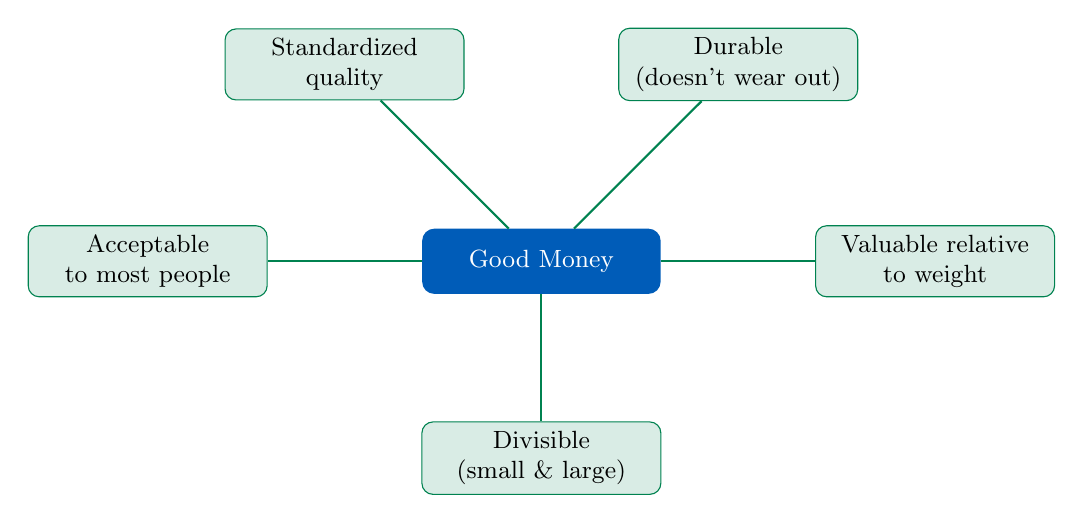
\begin{tikzpicture}[node distance=1.5cm, every node/.style={font=\small}]
\node[draw=accent, fill=accent, text=white, rounded corners, thick,
      minimum width=3cm, minimum height=0.8cm, align=center]
  (centre) at (0,0) {Good Money};
\node[draw=leafgreen, fill=leafgreen!15, rounded corners, text width=2.8cm, align=center]
  (acc) at (-5,0) {Acceptable\\to most people};
\node[draw=leafgreen, fill=leafgreen!15, rounded corners, text width=2.8cm, align=center]
  (std) at (-2.5,2.5) {Standardized\\quality};
\node[draw=leafgreen, fill=leafgreen!15, rounded corners, text width=2.8cm, align=center]
  (dur) at (2.5,2.5) {Durable\\(doesn't wear out)};
\node[draw=leafgreen, fill=leafgreen!15, rounded corners, text width=2.8cm, align=center]
  (val) at (5,0) {Valuable relative\\to weight};
\node[draw=leafgreen, fill=leafgreen!15, rounded corners, text width=2.8cm, align=center]
  (div) at (0,-2.5) {Divisible\\(small \& large)};
\draw[leafgreen, thick] (centre)--(acc);
\draw[leafgreen, thick] (centre)--(std);
\draw[leafgreen, thick] (centre)--(dur);
\draw[leafgreen, thick] (centre)--(val);
\draw[leafgreen, thick] (centre)--(div);
\end{tikzpicture}
\end{center}
\end{frame}

% ============================================================
\section{10.2 How Is Money Measured in Canada Today?}
% ============================================================

\begin{frame}{10.2 Learning Objective}
\transfade
\begin{block}{Goal}
Discuss the definitions of the money supply used in Canada today.
\end{block}
\begin{itemize}
  \item Different assets vary in \textbf{liquidity} (ease of conversion to spending).
  \item The Bank of Canada defines multiple \textbf{monetary aggregates}, from narrow to broad.
  \item \textbf{2024 approximate values (Bank of Canada):}
  \begin{itemize}
    \item M1+: $\approx \$1.2$ trillion
    \item M2: $\approx \$2.3$ trillion
    \item M2+: $\approx \$3.5$ trillion
  \end{itemize}
\end{itemize}
\end{frame}

\begin{frame}{Figure 10.1 -- Canada's Monetary Aggregates (2024)}
\begin{center}
\begin{tikzpicture}
\begin{axis}[
  width=0.80\textwidth, height=0.70\textheight,
  xbar stacked,
  bar width=0.8cm,
  xlabel={Size (\$billions)},
  symbolic y coords={M3,{M2++},{M2+},M2,{M1++},{M1+}},
  ytick=data,
  xmin=0, xmax=4200,
  tick label style={font=\small},
  label style={font=\small},
  title style={font=\small\bfseries},
  title={Bank of Canada Monetary Aggregates (approx.\ 2024, \$B)},
  enlarge y limits=0.15,
  legend style={at={(0.98,0.02)}, anchor=south east, font=\tiny},
  legend columns=2
]
\addplot[fill=accent!80, draw=accent] coordinates
  {(1200,{M1+})(1500,{M1++})(1500,M2)(1500,{M2+})(1500,{M2++})(1500,M3)};
\addplot[fill=leafgreen!70, draw=leafgreen] coordinates
  {(0,{M1+})(300,{M1++})(800,M2)(800,{M2+})(800,{M2++})(800,M3)};
\addplot[fill=goldenrod!70, draw=goldenrod] coordinates
  {(0,{M1+})(0,{M1++})(0,M2)(1200,{M2+})(1200,{M2++})(900,M3)};
\addplot[fill=deeporange!70, draw=deeporange] coordinates
  {(0,{M1+})(0,{M1++})(0,M2)(0,{M2+})(600,{M2++})(0,M3)};
\legend{Currency + chequable deposits, Non-chequable deposits,
        Non-bank deposits + MMFs, CSBs + non-MMFs}
\end{axis}
\end{tikzpicture}
\end{center}
{\tiny Source: Bank of Canada Banking and Financial Statistics, 2024. Values approximate.}
\end{frame}

\begin{frame}{Canada's Money Supply Measures Explained}
\transfade
\begin{center}
\small
\begin{tabular}{p{0.12\linewidth} p{0.80\linewidth}}
\toprule
\textbf{Measure} & \textbf{What It Includes} \\
\midrule
\textbf{M1+} & Currency in circulation + chequable deposits at banks, trust companies, credit unions. \textit{Most liquid.} \\
\textbf{M1++} & M1+ + non-chequable notice deposits. \\
\textbf{M2} & Currency + personal and non-personal deposits at banks. \\
\textbf{M2+} & M2 + deposits at trust/mortgage companies, credit unions (\textit{caisses populaires}), MMFs, life insurance annuities. \\
\textbf{M2++} & M2+ + Canada Savings Bonds + non-money market mutual funds. \textit{Broadest.} \\
\textbf{M3} & M2 + non-personal term deposits + foreign-currency deposits. \\
\bottomrule
\end{tabular}
\end{center}
\vspace{0.3em}
\begin{itemize}
  \item For most macroeconomic analysis, \textbf{M1+} is most relevant (transactions money).
\end{itemize}
\end{frame}

% ============================================================
\section{10.3 How Do Banks Create Money?}
% ============================================================

\begin{frame}{10.3 Learning Objective}
\transfade
\begin{block}{Goal}
Explain how banks create money.
\end{block}
\begin{itemize}
  \item \textbf{How can banks create money?}
  \begin{itemize}
    \item They accept deposits and make loans.
    \item Loans create new deposits --- the money supply \alert{expands}.
  \end{itemize}
  \item \textbf{Canada's major banks (Big Six):}
  \begin{itemize}
    \item Royal Bank (RBC), TD Bank, Scotiabank, BMO, CIBC, National Bank.
    \item Combined assets $\approx \$8$ trillion (2024) --- one of the most concentrated banking systems in the world.
  \end{itemize}
  \item Banks in Canada are not legally required to hold a specific reserve ratio (unlike the U.S.).
  \item They set their own \textbf{desired reserve ratio} ($r_d$) based on liquidity needs.
\end{itemize}
\end{frame}

\begin{frame}{Bank Balance Sheets: A T-Account Example}
\transfade
\begin{itemize}
  \item You deposit \alert{\$1{,}000} in cash at RBC.
\end{itemize}
\vspace{0.3em}
\begin{center}
\begin{tabular}{p{0.45\linewidth} p{0.45\linewidth}}
\toprule
\multicolumn{2}{c}{\textbf{Royal Bank --- T-Account}} \\
\midrule
\textbf{Assets} & \textbf{Liabilities} \\
\midrule
Reserves $+\$1{,}000$ & Deposits (chequing) $+\$1{,}000$ \\
\bottomrule
\end{tabular}
\end{center}
\vspace{0.5em}
\begin{itemize}
  \item \textbf{Note:} currency in circulation fell by \$1{,}000, but chequing deposits rose by \$1{,}000.
  \item Total money supply is \textbf{unchanged so far}.
  \item But now RBC can lend!
\end{itemize}
\end{frame}

\begin{frame}{From Deposits to Loans: Creating New Money}
\transfade
\begin{itemize}
  \item Suppose RBC keeps 10\% ($r_d = 0.10$) as reserves and lends \alert{\$900}.
\end{itemize}
\begin{center}
\small
\begin{tabular}{p{0.45\linewidth} p{0.45\linewidth}}
\toprule
\multicolumn{2}{c}{\textbf{RBC --- After Making Loan}} \\
\midrule
\textbf{Assets} & \textbf{Liabilities} \\
\midrule
Reserves $+\$100$ & Deposits $+\$1{,}000$ \\
Loan $+\$900$ & \\
\bottomrule
\end{tabular}
\end{center}
\vspace{0.4em}
\begin{itemize}
  \item The \$900 loan is spent by the borrower and deposited at TD Bank.
  \item TD now has \$900 in new deposits, keeps \$90, lends \$810.
  \item \$810 ends up at Scotiabank --- and the process continues.
  \item This is the \textbf{money creation process}.
\end{itemize}
\end{frame}

\begin{frame}{Figure 10.2 -- Multiple Rounds of Money Creation}
\begin{center}
\begin{tikzpicture}
\begin{axis}[
  width=0.82\textwidth, height=0.68\textheight,
  ybar, bar width=0.8cm,
  xlabel={Round of Lending},
  ylabel={New Deposits Created (\$)},
  symbolic x coords={Round 1,Round 2,Round 3,Round 4,Round 5,Round 6+},
  xtick=data,
  ymin=0, ymax=1100,
  nodes near coords,
  nodes near coords style={font=\tiny},
  tick label style={font=\small},
  label style={font=\small},
  title style={font=\small\bfseries},
  title={Each Round Creates Less Money ($r_d = 10\%$, Initial Deposit = \$1{,}000)},
  enlarge x limits=0.08
]
\addplot[fill=accent!70, draw=accent] coordinates {
  (Round 1,1000)(Round 2,900)(Round 3,810)(Round 4,729)(Round 5,656)(Round 6+,4905)
};
\end{axis}
\end{tikzpicture}
\end{center}
{\tiny Total deposits $= \frac{1}{r_d} \times \$1{,}000 = \frac{1}{0.10} \times \$1{,}000 = \$10{,}000$. Banking system created \$9{,}000 of new money.}
\end{frame}

\begin{frame}{The Simple Deposit Multiplier}
\transfade
\begin{itemize}
  \item \textbf{Simple deposit multiplier:}
  \[
    \text{Total deposits} = \frac{1}{r_d} \times \Delta \text{Reserves}.
  \]
  \[
    \text{Simple deposit multiplier} = \frac{1}{r_d}.
  \]
  \item \textbf{Examples:}
  \begin{itemize}
    \item $r_d = 10\%$: multiplier $= 10$.
    \item $r_d = 5\%$: multiplier $= 20$.
    \item $r_d = 20\%$: multiplier $= 5$.
  \end{itemize}
  \item \textbf{Real-world multiplier is smaller} because:
  \begin{enumerate}
    \item Banks hold excess reserves (especially during crises).
    \item Some loans are held as cash, not redeposited.
  \end{enumerate}
  \item \textbf{Canadian example (2020):} BoC emergency lending boosted bank reserves, but banks were cautious --- real multiplier stayed low as lending was slow to respond.
\end{itemize}
\end{frame}

% ============================================================
\section{10.5 The Quantity Theory of Money}
% ============================================================

\begin{frame}{10.5 Learning Objective}
\transfade
\begin{block}{Goal}
Explain the quantity theory of money and use it to explain how high inflation occurs.
\end{block}
\begin{itemize}
  \item The \textbf{quantity equation} (Irving Fisher, early 1900s):
  \[
    M \times V = P \times Y,
  \]
  where:
  \begin{itemize}
    \item $M$ = money supply,
    \item $V$ = velocity of money (how often each dollar is spent per year),
    \item $P$ = price level,
    \item $Y$ = real GDP.
  \end{itemize}
  \item Note: $P \times Y = $ \textbf{nominal GDP}.
\end{itemize}
\end{frame}

\begin{frame}{The Quantity Theory: Key Assumptions}
\transfade
\begin{itemize}
  \item \textbf{Quantity theory of money:} assumes $V$ is approximately constant in the long run.
  \item With $V$ constant, changes in $M$ must affect $P \times Y$.
  \item In growth-rate form:
  \[
    g_M + g_V = \pi + g_Y.
  \]
  \item If $g_V \approx 0$:
  \[
    g_M = \pi + g_Y \quad \Rightarrow \quad \boxed{\pi = g_M - g_Y}.
  \]
  \item \textbf{Implication:} inflation is a \textbf{monetary phenomenon} in the long run.
  \begin{itemize}
    \item If money grows faster than real output $\Rightarrow$ inflation.
    \item If money grows at the same rate as real output $\Rightarrow$ stable prices.
  \end{itemize}
\end{itemize}
\end{frame}

\begin{frame}{Figure 10.3 -- Money Growth and Inflation (Canada 2010--2024)}
\begin{center}
\begin{tikzpicture}
\begin{axis}[
  width=0.88\textwidth, height=0.70\textheight,
  xlabel={Year},
  ylabel={Annual Growth Rate (\%)},
  xmin=2010, xmax=2025,
  ymin=-5, ymax=25,
  xtick={2010,2012,2014,2016,2018,2020,2022,2024},
  xticklabel style={rotate=45, anchor=east, font=\tiny},
  grid=both, grid style={dotted,gray!40},
  tick label style={font=\tiny},
  label style={font=\small},
  legend pos=north west,
  legend style={font=\tiny},
  title style={font=\small\bfseries},
  title={Money Supply Growth Led Inflation with a Lag (Canada)}
]
% M1+ growth (approximate)
\addplot[accent, very thick, mark=*, mark size=1.5pt] coordinates {
  (2010,9)(2011,7)(2012,6)(2013,5)(2014,4)(2015,5)(2016,6)
  (2017,5)(2018,4)(2019,5)(2020,20)(2021,18)(2022,5)(2023,2)(2024,3)
};
% CPI inflation (approximate)
\addplot[canadared, very thick, mark=square*, mark size=1.5pt] coordinates {
  (2010,1.8)(2011,2.9)(2012,1.5)(2013,0.9)(2014,1.9)(2015,1.1)(2016,1.4)
  (2017,1.6)(2018,2.3)(2019,1.9)(2020,0.7)(2021,3.4)(2022,6.8)(2023,3.9)(2024,2.7)
};
\legend{M1+ growth (\%), CPI Inflation (\%)}
\node[font=\tiny, fill=soft, draw=accent, rounded corners, align=center]
  at (axis cs:2021,22) {COVID M1+\\surge (+20\%)};
\node[font=\tiny, fill=lightred, draw=canadared, rounded corners, align=center]
  at (axis cs:2022.5,9) {Inflation\\surged 2 yrs\\later};
\end{axis}
\end{tikzpicture}
\end{center}
{\tiny Sources: Bank of Canada; Statistics Canada. M1+ and CPI data, annual averages.}
\end{frame}

\begin{frame}{Hyperinflation: Money Growth Gone Wrong}
\transfade
\begin{itemize}
  \item \textbf{Hyperinflation:} inflation exceeding \alert{50\% per month}.
  \item Caused by governments printing money to finance large budget deficits.
  \item \textbf{Historical examples:}
  \begin{itemize}
    \item \textbf{Germany 1923:} prices doubled every 3.7 days --- workers demanded to be paid twice daily and immediately spent wages.
    \item \textbf{Zimbabwe 2008:} inflation reached $5 \times 10^{10}$\% per month; the government issued 100 trillion dollar bills.
    \item \textbf{Venezuela 2018:} $\approx$1{,}000{,}000\% annual inflation; many Venezuelans switched to USD or Bitcoin.
  \end{itemize}
  \item \textbf{Lesson for Canada:} Bank of Canada independence and the 2\% inflation target prevent excessive money printing. \textcolor{leafgreen}{This institutional framework matters enormously.}
\end{itemize}
\end{frame}

\begin{frame}{Figure 10.4 -- Quantity Theory: Cross-Country Evidence}
\begin{center}
\begin{tikzpicture}
\begin{axis}[
  width=0.80\textwidth, height=0.68\textheight,
  xlabel={Average Money Growth Rate (\%, 5-yr avg.)},
  ylabel={Average Inflation Rate (\%)},
  xmin=0, xmax=25, ymin=0, ymax=22,
  grid=both, grid style={dotted,gray!40},
  tick label style={font=\small},
  label style={font=\small},
  title style={font=\small\bfseries},
  title={Countries with Higher Money Growth Have Higher Inflation}
]
% 45-degree reference line
\addplot[gray, dashed, thick, domain=0:25] {x - 2}
  node[right, font=\tiny] {$\pi = g_M - g_Y$};
% Country data points (schematic)
\addplot[only marks, mark=*, mark size=3pt, accent] coordinates {
  (2,1.5)(3,2.0)(2.5,1.8)(4,2.5)(5,3.5)(6,4.5)
  (8,6)(10,8)(12,10.5)(15,14)(18,17)(22,20)
};
\node[font=\tiny] at (axis cs:3,3.5) {Canada};
\node[font=\tiny] at (axis cs:5,5) {USA};
\node[font=\tiny] at (axis cs:10,9) {Brazil};
\node[font=\tiny] at (axis cs:15,15) {Turkey};
\node[font=\tiny] at (axis cs:22,21) {Venezuela};
\node[font=\tiny, fill=soft, draw=accent, rounded corners, align=center]
  at (axis cs:7,18) {Strong positive\\relationship,\\especially at\\high inflation};
\end{axis}
\end{tikzpicture}
\end{center}
{\tiny Schematic illustration based on cross-country monetary data. High-inflation countries have high money growth.}
\end{frame}

\begin{frame}{Quantity Theory: Main Takeaways}
\transfade
\begin{itemize}
  \item The quantity theory is primarily a \textbf{long-run} theory.
  \item \textbf{Sustained inflation requires sustained money growth exceeding real GDP growth.}
  \item \textbf{Canada's COVID experience:}
  \begin{itemize}
    \item M1+ grew $\approx$20\% in 2020--21 (emergency pandemic liquidity).
    \item Real GDP growth was modest ($\approx$5\% recovery).
    \item Result: excess money growth contributed to the 2021--22 inflation surge.
    \item \textcolor{goldenrod}{Source: Bank of Canada, Banking and Financial Statistics.}
  \end{itemize}
  \item \textbf{Bank of Canada's response:} reduce money supply growth AND raise overnight rate --- consistent with both the quantity theory and the AD-AS framework.
\end{itemize}
\end{frame}

% ============================================================
\section*{Chapter Summary}
% ============================================================

\begin{frame}{Summary}
\transfade
\begin{itemize}
  \item \textbf{Money} is any widely accepted asset. It performs four functions:
  \begin{itemize}
    \item medium of exchange, unit of account, store of value, standard of deferred payment.
  \end{itemize}
  \item Canada uses fiat money; the Bank of Canada controls the money supply.
  \item Monetary aggregates (M1+, M2, M2++) measure different degrees of liquidity.
  \item Banks \textbf{create money} by accepting deposits and making loans:
  \[
    \text{Simple deposit multiplier} = \frac{1}{r_d}.
  \]
  \item Real-world multiplier is smaller due to excess reserves and cash holdings.
  \item The \textbf{quantity theory} ($\pi = g_M - g_Y$) predicts that persistent inflation requires persistent excess money growth.
  \item Canada's 2020--22 M1+ surge contributed to the worst inflation since the 1980s --- tamed by the BoC's 2022--24 rate hiking cycle.
\end{itemize}
\end{frame}

\begin{frame}
\centering
\Huge \textbf{Thank you!}\\[1em]
\large Questions?
\end{frame}

\end{document}
